\chapter{Results}
\label{chap:5}
%
We plot the mean and the standard deviation of the cumulative reward for all kernel runs. One kernel run consists of a number of trials depending on the experiment. We use more than one trial per kernel to compensate for the variable result one run can produce. Also, due to high variations between iteration steps, all plots are smoothed by a moving mean of 15 steps. And the standard deviation values are divided by five to maintain readability when three or four different kernel plots are present in one graph. Each plot includes the mean of every kernel's outcome as a line and the corresponding standard deviation as a shaded area above and below. The green and blue graph show the two standard kernels, squared exponential and Matérn 5/2, and the magenta and red graph show the trajectory kernels. The trajectory kernel proposed by \cite{wilson2014using} is marked as the magenta one, whereas the trajectory kernel we come up with (Section \ref{sec:ownTK}) is marked as the red one. Also a table is provided for each experiment showing the benchmark data for corresponding kernels. The column \textbf{mean(time)} contains the mean value of the minutes needed for each trail and the column \textbf{std(time)} the associated standard deviation. The column \textbf{time performance} relates the time needed for the whole run to the time needed for the squared exponential kernel run. If the percentage is negative the associated kernel took more time than the squared exponential kernel. The last column, \textbf{learning performance}, compares the summarized cumulative rewards to those of the squared exponential kernel. If the percentage is positive then the overall learning performance is better than the squared exponential kernel ones. The discrete version of the OpenAI Gym Mountain Car ('MountainCar-v0') stayed at the lowest possible reward during all experiments, therefore we plot no results.

\begin{table}[h]
    \centering
    \begin{tabular}{|l|l|l|l|l|}\hline
        Environment & Optimizer & Action space & Kernels & Simulation\\\hline
        Cart Pole & globally & continuous & S, M, TW, TO & MATLAB (cluster)\\\hline
        Cart Pole & locally & continuous & S, M, TO & MATLAB (cluster)\\\hline
        Cart Pole & locally & discrete & S, M, TO & OpenAI Gym (laptop)\\\hline
        Acrobot & locally & discrete & S, M, TO & OpenAI Gym (laptop)\\\hline
        Mountain Car & locally & continuous & S, M, TO & OpenAI Gym (laptop)\\\hline
    \end{tabular}
    \caption{Overview of all performance experiments. The abbreviations in the column kernels stand for: S = squared exponential, M = Matérn 5/2, TW = trajectory (Wilson 2014), TO = trajectory (own work). The part of the TU Darmstadt cluster we used for parallel runs is equipped with Intel Xeon E5-4650 processors with 2.7 GHz each. The runs involving the OpenAI Gym were performed on my laptop's Intel Core i5-7200U processor operating at 2.5 GHz.\label{table:xps}}
\end{table}

\newpage
\section{Learning performance}

Here we plot the learning performance of each experiment. We also provide tables with corresponding benchmark data.

\subsection{Cart pole}
This subsection contains the results of the different Cart Pole setups.

\subsubsection{MATLAB implementation of Cart pole on the global optimizer}

In figure \ref{fig:cartpoleMatlabGlobal} we plot four different kernel runs of the MATLAB CartPole implementation in the global Bayesian optimization context. Our MATLAB CartPole implementation runs at most until 1000 time steps. For this implementation we use a continuous action selection policy with four dimensions. Ten trials were completed on each kernel to observe the average performance.

\begin{figure}[h]
    \centering
    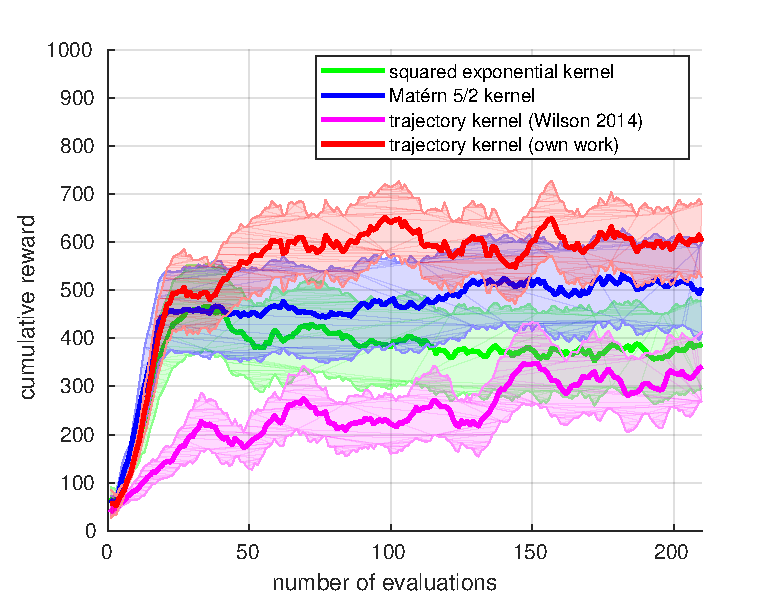
\includegraphics[width=.7\textwidth]{/home/sebastian/Documents/bscThesis/img/results/global_cartpole_matlab_10.pdf}
    \caption{Results of the MATLAB Cart Pole implementation with a continuous action selection policy with the global optimization. Each kernel graph contains the average over 10 trials.}
    \label{fig:cartpoleMatlabGlobal}
\end{figure}
\begin{table}[h]
    \centering
    % \begin{tabular}{|l|r|r|r|r|r|r|}\hline
    %     kernel & mean(time) & std(time) & time & learning & \multicolumn{2}{c|}{standard deviation}\\
    %     & & & performance & performance & ($\sigma_f$) & ($\sigma_l$)\\\hline
    \begin{tabular}{|l|r|r|r|r|}\hline
        kernel & mean(time) & std(time) & time performance & learning performance\\\hline
        squared exponential & 17 min & 5 min & 0 \% & 0 \%\\\hline
        Matérn 5/2 & 18 min & 4 min & -5 \% & +23 \%\\\hline
        trajectory (Wilson 2014) & 150 min & 48 min & -769 \% & -35 \%\\\hline
        trajectory (own work) & 393 min & 51 min & -2187 \% & +47 \%\\\hline
    \end{tabular}
    \caption{Performance of different kernels on the MATLAB Cart Pole implementation with the global optimizer.\label{table:cartpoleMatlabGlobal}}
\end{table}


\newpage
\subsubsection{MATLAB implementation of Cart pole on the local optimizer}
In figure \ref{fig:cartpoleMatlabLocal} we plot three different kernel runs of the MATLAB CartPole implementation in the local Bayesian optimization context. For this implementation we use a continuous action selection policy with four dimensions. Ten trials were completed on each kernel to observe the average performance.

\begin{figure}[h]
    \centering
    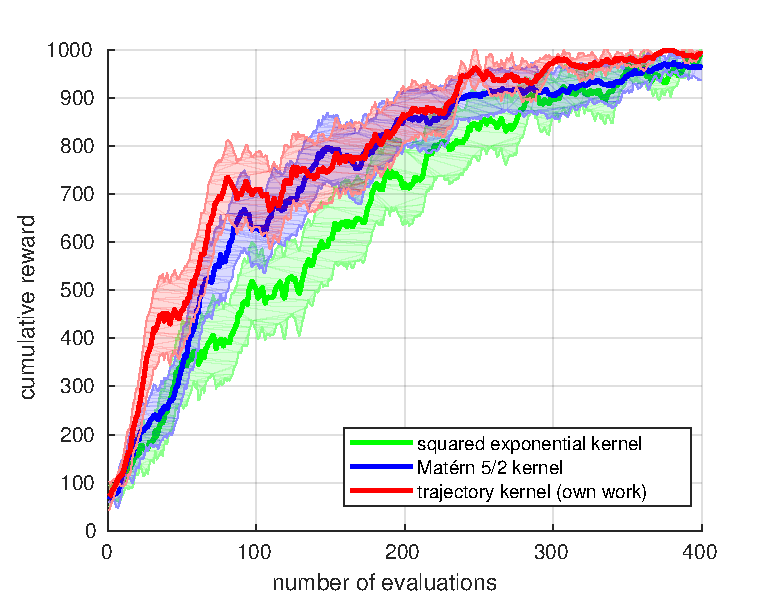
\includegraphics[width=0.7\textwidth]{/home/sebastian/Documents/bscThesis/img/results/local_cartpole_matlab_10.pdf}
    \caption{Results of the MATLAB Cart Pole implementation with a continuous action selection policy on the local optimizer. Each kernel graph contains the average over 10 trials.}
    \label{fig:cartpoleMatlabLocal}
\end{figure}
\begin{table}[h]
    \centering
    \begin{tabular}{|l|r|r|r|r|}\hline
        kernel & mean(time) & std(time) & time performance & learning performance\\\hline
        squared exponential & 9 min & 1 min & 0 \% & 0 \%\\\hline
        Matérn 5/2 & 10 min & 1 min & -13 \% & +11 \%\\\hline
        trajectory (own work) & 30 min & 1 min & -235 \% & +18 \%\\\hline
    \end{tabular}
    \caption{Performance of different kernels on the MATLAB Cart Pole implementation on the local Bayesian optimizer.\label{table:matlab_cartpole_local}}
\end{table}

\newpage
\subsubsection{OpenAI Gym implementation of Cart pole on the local optimizer}
In figure \ref{fig:cartpolePygym} we plot three different kernel runs of the OpenAI Gym CartPole implementation in the local Bayesian optimization context. For this implementation we use a discrete action selection policy with five dimensions for two possible actions resulting in a total of ten dimensions. Ten trials were completed on each kernel to observe the average performance.

\begin{figure}[h]
    \centering
    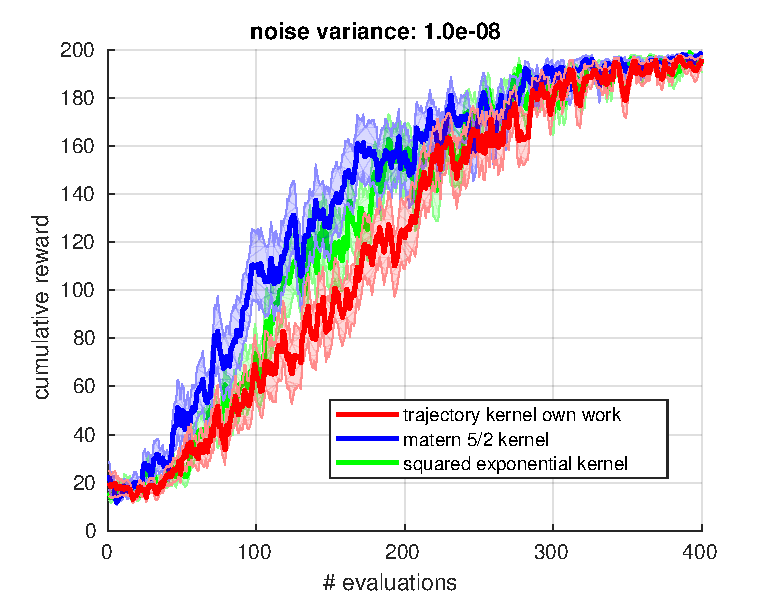
\includegraphics[width=0.7\textwidth]{/home/sebastian/Documents/bscThesis/img/results/local_cartpole_pygym_10.pdf}
    \caption{Results of the OpenAI Gym Cart Pole implementation with a discrete action selection policy on the local optimizer. Each kernel graph contains the average over 10 trials.}
    \label{fig:cartpolePygym}
\end{figure}
\begin{table}[h]
    \centering
    \begin{tabular}{|l|r|r|r|r|}\hline
        kernel & mean(time) & std(time) & time performance & learning performance\\\hline
        squared exponential & 6 min & 1 min & 0 \% & 0 \%\\\hline
        Matérn 5/2 & 9 min & 1 min & -37 \% & +7 \%\\\hline
        trajectory (own work) & 62 min & 3 min & -861 \% & -8 \%\\\hline
    \end{tabular}
    \caption{Performance of different kernels on the OpenAI Cart Pole on the local optimizer.\label{table:pygym_cartpole_local}}
\end{table}

\newpage
\subsection{Acrobot}
In figure \ref{fig:acrobotPygym} we plot three different kernel runs of the OpenAI Gym Acrobot implementation in the local Bayesian optimization context. For this implementation we use a discrete action selection policy with seven dimensions for three possible actions resulting in a total of 21 dimensions. Ten trials were completed on each kernel to observe the average performance.
\begin{figure}[h]
    \centering
    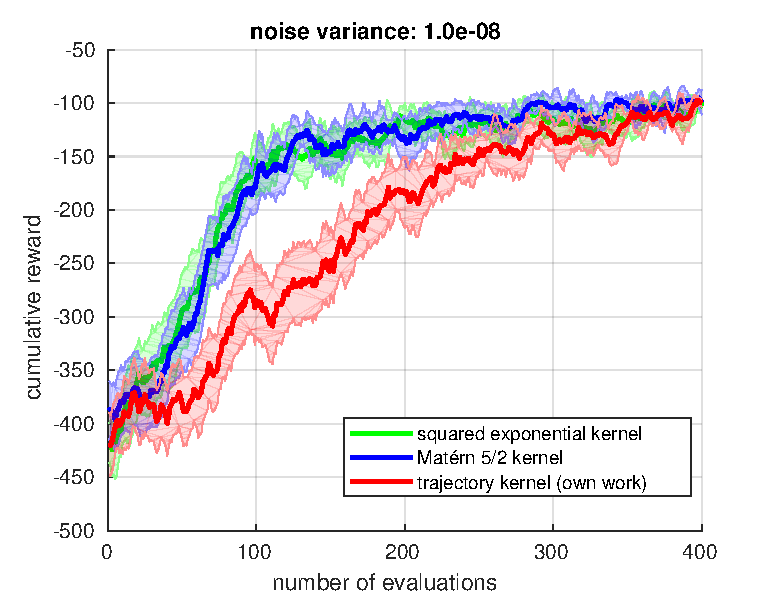
\includegraphics[width=0.7\textwidth]{/home/sebastian/Documents/bscThesis/img/results/local_acrobot_pygym_10.pdf}
    \caption{Results of the OpenAI Gym Acrobot implementation with a discrete action selection policy on the local optimizer. Each kernel graph contains the average over 10 trials.}
    \label{fig:acrobotPygym}
\end{figure}
\begin{table}[h]
    \centering
    \begin{tabular}{|l|r|r|r|r|}\hline
        kernel & mean(time) & std(time) & time performance & learning performance\\\hline
        squared exponential & 7 min & 0 min & 0 \% & 0 \%\\\hline
        Matérn 5/2 & 8 min & 1 min & -12 \% & +1 \%\\\hline
        trajectory (own work) & 70 min & 5 min & -923 \% &-32 \%\\\hline
    \end{tabular}
    \caption{Performance of different kernels on the OpenAI Gym Acrobot on the local optimizer.\label{table:pygym_cartpole_local}}
\end{table}

\newpage
\subsection{Mountain Car}
In figure \ref{fig:mountaincarPygym} we plot three different kernel runs of the OpenAI Gym Mountain Car continuous implementation in the local Bayesian optimization context. For this implementation we use a continuous action selection policy with ten dimensions. Ten trials were completed on each kernel to observe the average performance.
\begin{figure}[h]
    \centering
    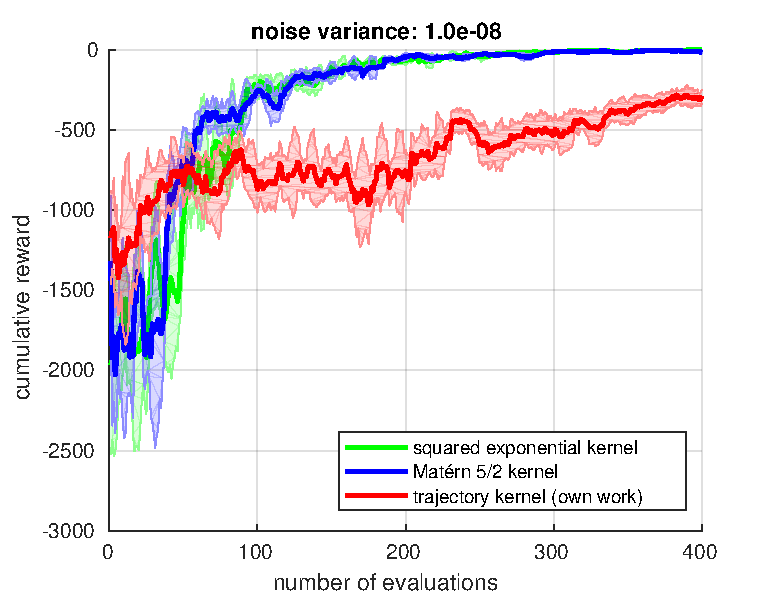
\includegraphics[width=0.7\textwidth]{/home/sebastian/Documents/bscThesis/img/results/local_mountaincar_pygym_10.pdf}
    \caption{Results of the OpenAI Gym Mountain Car continuous implementation with a continuous action selection policy on the local optimizer. Each kernel graph contains the average over 10 trials.}
    \label{fig:mountaincarPygym}
\end{figure}
\begin{table}[h]
    \centering
    \begin{tabular}{|l|r|r|r|r|}\hline
        kernel & mean(time) & std(time) & time performance & learning performance\\\hline
        squared exponential & 1 min & 0 min & 0 \% & 0 \%\\\hline
        Matérn 5/2 & 1 min & 0 min & -25 \% & +10 \%\\\hline
        trajectory (own work) & 101 min & 6 min & -12728 \% & -103 \%\\\hline
    \end{tabular}
    \caption{Performance of different kernels on the OpenAI Gym Mountain Car continuous on the local optimizer.\label{table:pygym_cartpole_local}}
\end{table}




\newpage
\section{Sensitivity analysis}
\begin{figure}[H]
\centering
%\vspace{-3cm}
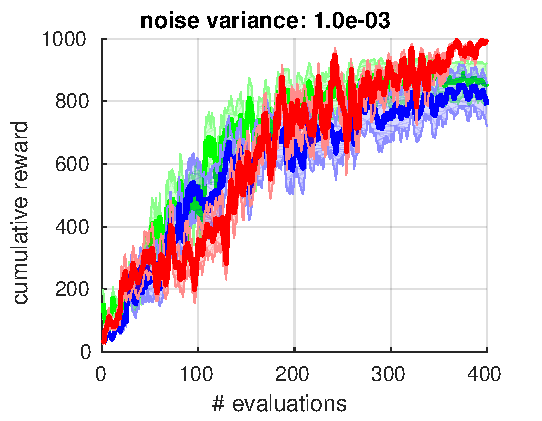
\includegraphics[width=0.4\textwidth]{/home/sebastian/Documents/bscThesis/img/noisecompare/1.pdf}
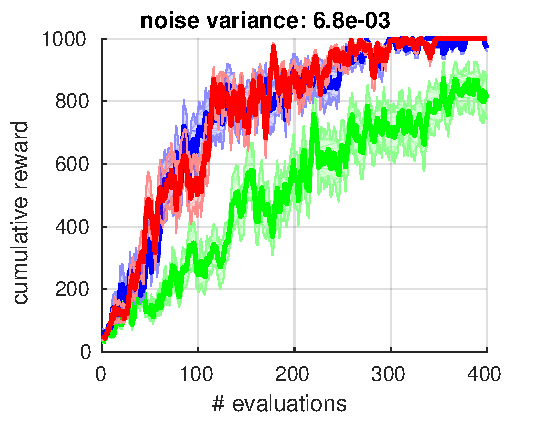
\includegraphics[width=0.4\textwidth]{/home/sebastian/Documents/bscThesis/img/noisecompare/2.pdf}
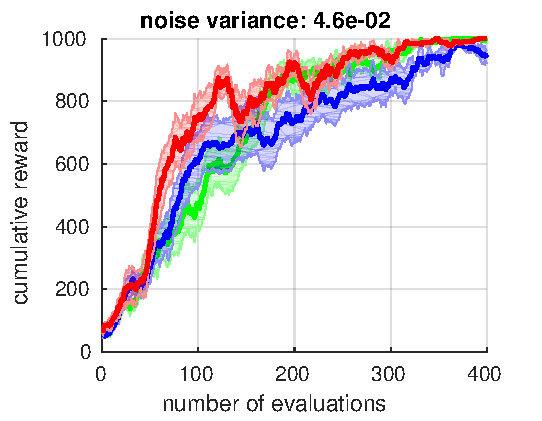
\includegraphics[width=0.4\textwidth]{/home/sebastian/Documents/bscThesis/img/noisecompare/3.pdf}
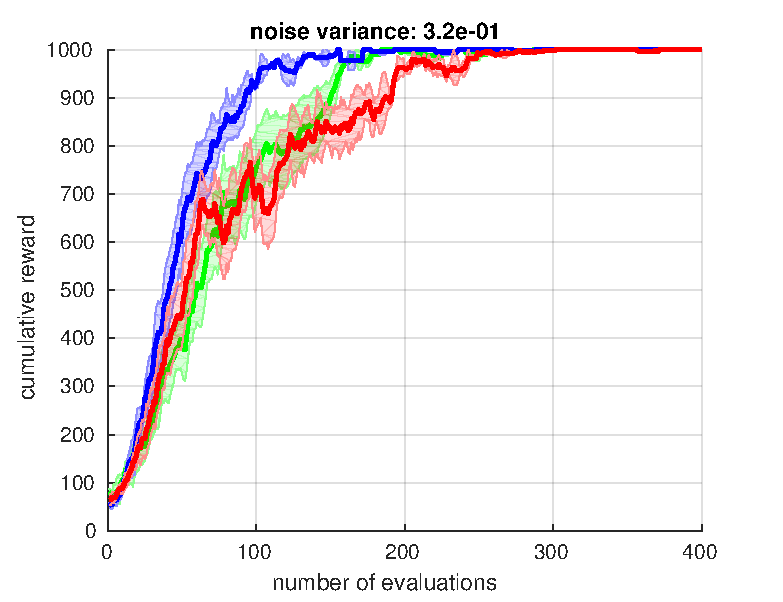
\includegraphics[width=0.4\textwidth]{/home/sebastian/Documents/bscThesis/img/noisecompare/4.pdf}
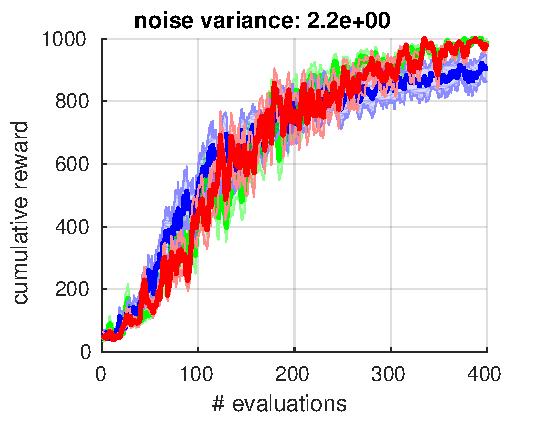
\includegraphics[width=0.4\textwidth]{/home/sebastian/Documents/bscThesis/img/noisecompare/5.pdf}
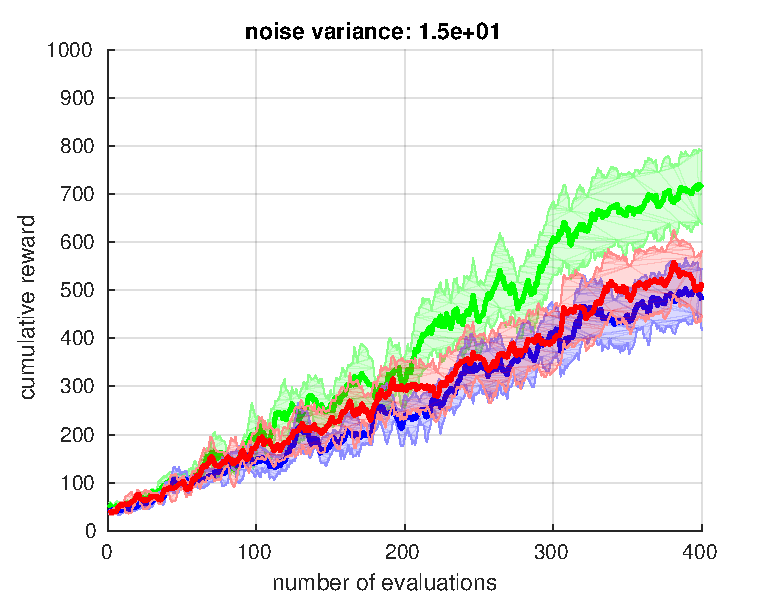
\includegraphics[width=0.4\textwidth]{/home/sebastian/Documents/bscThesis/img/noisecompare/6.pdf}
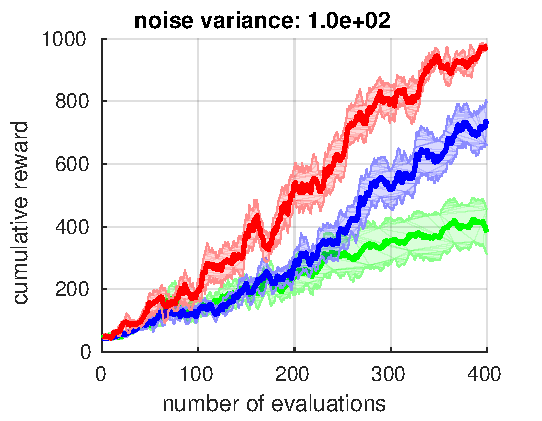
\includegraphics[width=0.4\textwidth]{/home/sebastian/Documents/bscThesis/img/noisecompare/7.pdf}
\raisebox{\height}{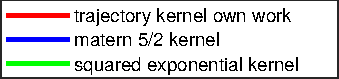
\includegraphics[width=0.4\textwidth]{/home/sebastian/Documents/bscThesis/img/noisecompare/legend.pdf}}
\caption{Noise level comparison on the MATLAB Cart Pole implementation with 1000 time steps on the local Bayesian optimizer. The noise levels are logarithmically spaced and sorted in ascending order from $10^{-3}$ to $10^2$. Each kernel graph contains the average over 5 trials.}
\label{fig:noisecompare}
\end{figure}
